

\tikzset{every picture/.style={line width=0.75pt}} %set default line width to 0.75pt        

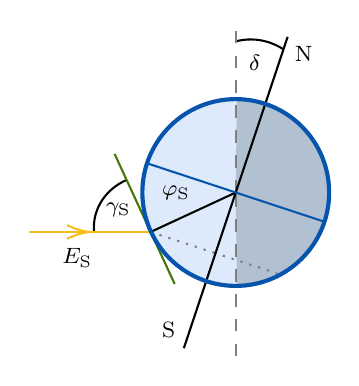
\begin{tikzpicture}[x=0.75pt,y=0.75pt,yscale=-1,xscale=1]
%uncomment if require: \path (0,181); %set diagram left start at 0, and has height of 181

%Shape: Arc [id:dp1509931683753729] 
\draw  [draw opacity=0] (41.51,107.98) .. controls (41.44,107.22) and (41.4,106.45) .. (41.4,105.68) .. controls (41.4,95.62) and (47.84,86.94) .. (57.17,82.86) -- (69.17,105.68) -- cycle ; \draw   (41.51,107.98) .. controls (41.44,107.22) and (41.4,106.45) .. (41.4,105.68) .. controls (41.4,95.62) and (47.84,86.94) .. (57.17,82.86) ;
%Shape: Pie [id:dp008234319355738817] 
\draw  [color={rgb, 255:red, 0; green, 0; blue, 0 }  ,draw opacity=0 ][fill={rgb, 255:red, 0; green, 0; blue, 0 }  ,fill opacity=0.45 ] (110.26,43.91) .. controls (135.04,44.18) and (155.08,64.13) .. (155.16,88.77) .. controls (155.24,113.51) and (135.17,133.66) .. (110.25,133.93) -- (109.75,88.92) -- cycle ;
%Shape: Circle [id:dp3321431212746069] 
\draw  [color={rgb, 255:red, 7; green, 84; blue, 173 }  ,draw opacity=1 ][fill={rgb, 255:red, 200; green, 222; blue, 248 }  ,fill opacity=0.64 ][line width=0.75]  (64.75,88.92) .. controls (64.75,64.07) and (84.9,43.92) .. (109.75,43.92) .. controls (134.6,43.92) and (154.75,64.07) .. (154.75,88.92) .. controls (154.75,113.77) and (134.6,133.92) .. (109.75,133.92) .. controls (84.9,133.92) and (64.75,113.77) .. (64.75,88.92) -- cycle ;
%Straight Lines [id:da8319048303736489] 
\draw [color={rgb, 255:red, 65; green, 117; blue, 5 }  ,draw opacity=1 ]   (57.17,82.86) -- (68.75,107.92) ;
%Shape: Arc [id:dp7416942399851174] 
\draw  [draw opacity=0] (109.46,16.18) .. controls (111.99,15.49) and (114.61,15.14) .. (117.3,15.17) .. controls (122.89,15.24) and (128.16,16.96) .. (132.83,19.97) -- (116.75,59.92) -- cycle ; \draw   (109.46,16.18) .. controls (111.99,15.49) and (114.61,15.14) .. (117.3,15.17) .. controls (122.89,15.24) and (128.16,16.96) .. (132.83,19.97) ;
%Straight Lines [id:da23785833539369183] 
\draw [color={rgb, 255:red, 128; green, 128; blue, 128 }  ,draw opacity=1 ] [dash pattern={on 4.5pt off 4.5pt}]  (109.75,167.84) -- (109.75,88.92) ;
%Straight Lines [id:da06972248148475568] 
\draw [color={rgb, 255:red, 128; green, 128; blue, 128 }  ,draw opacity=1 ] [dash pattern={on 4.5pt off 4.5pt}]  (109.75,88.92) -- (109.75,10) ;
%Straight Lines [id:da8960602024330377] 
\draw [line width=0.75]    (68.75,107.92) -- (109.75,88.92) ;
%Straight Lines [id:da5098060920131091] 
\draw [color={rgb, 255:red, 128; green, 128; blue, 128 }  ,draw opacity=1 ] [dash pattern={on 0.84pt off 2.51pt}]  (99.25,117.92) -- (129.75,127.92) ;
%Straight Lines [id:da8906380552334501] 
\draw [color={rgb, 255:red, 128; green, 128; blue, 128 }  ,draw opacity=1 ] [dash pattern={on 0.84pt off 2.51pt}]  (68.75,107.92) -- (99.25,117.92) ;
%Straight Lines [id:da14349690184184327] 
\draw    (109.75,88.92) -- (84.75,163.92) ;
%Straight Lines [id:da024036142327008347] 
\draw    (134.75,13.92) -- (109.75,88.92) ;
%Straight Lines [id:da21245027564913532] 
\draw [color={rgb, 255:red, 7; green, 84; blue, 173 }  ,draw opacity=1 ]   (67.25,74.92) -- (109.75,88.92) ;
%Straight Lines [id:da7748765899346521] 
\draw [color={rgb, 255:red, 7; green, 84; blue, 173 }  ,draw opacity=1 ]   (109.75,88.92) -- (152.25,102.92) ;
%Straight Lines [id:da645165483038932] 
\draw [color={rgb, 255:red, 65; green, 117; blue, 5 }  ,draw opacity=1 ]   (68.75,107.92) -- (80.33,132.98) ;
%Straight Lines [id:da01702325380082992] 
\draw [color={rgb, 255:red, 65; green, 117; blue, 5 }  ,draw opacity=1 ]   (57.17,82.86) -- (51.38,70.33) ;
%Straight Lines [id:da7674893611261671] 
\draw [color={rgb, 255:red, 248; green, 189; blue, 28 }  ,draw opacity=1 ]   (39.38,107.92) -- (68.75,107.92) ;
%Straight Lines [id:da5473156330354862] 
\draw [color={rgb, 255:red, 248; green, 189; blue, 28 }  ,draw opacity=1 ]   (10,107.92) -- (37.38,107.92) ;
\draw [shift={(39.38,107.92)}, rotate = 180] [color={rgb, 255:red, 248; green, 189; blue, 28 }  ,draw opacity=1 ][line width=0.75]    (10.93,-3.29) .. controls (6.95,-1.4) and (3.31,-0.3) .. (0,0) .. controls (3.31,0.3) and (6.95,1.4) .. (10.93,3.29)   ;
%Shape: Circle [id:dp46167221588038543] 
\draw  [color={rgb, 255:red, 7; green, 84; blue, 173 }  ,draw opacity=1 ][fill={rgb, 255:red, 200; green, 222; blue, 248 }  ,fill opacity=0 ][line width=1.5]  (64.75,88.92) .. controls (64.75,64.07) and (84.9,43.92) .. (109.75,43.92) .. controls (134.6,43.92) and (154.75,64.07) .. (154.75,88.92) .. controls (154.75,113.77) and (134.6,133.92) .. (109.75,133.92) .. controls (84.9,133.92) and (64.75,113.77) .. (64.75,88.92) -- cycle ;

% Text Node
\draw (72.75,84.32) node [anchor=north west][inner sep=0.75pt]  [font=\footnotesize]  {$\varphi _{\mathrm{S}}$};
% Text Node
\draw (114.75,21.32) node [anchor=north west][inner sep=0.75pt]  [font=\footnotesize]  {$\delta $};
% Text Node
\draw (45.75,92.32) node [anchor=north west][inner sep=0.75pt]  [font=\footnotesize]  {$\gamma _{\mathrm{S}}$};
% Text Node
\draw (24.75,114.32) node [anchor=north west][inner sep=0.75pt]  [font=\footnotesize]  {$E_{\mathrm{S}}$};
% Text Node
\draw (136.75,16.92) node [anchor=north west][inner sep=0.75pt]  [font=\footnotesize] [align=left] {N};
% Text Node
\draw (72.75,149.92) node [anchor=north west][inner sep=0.75pt]  [font=\footnotesize] [align=left] {S};


\end{tikzpicture}
